\documentclass[11pt,a4paper]{article}
\usepackage[utf8]{inputenc}
\usepackage[margin=1in]{geometry}
\usepackage{graphicx}
\usepackage{booktabs}
\usepackage{amsmath}
\usepackage{caption}
\usepackage{hyperref}
\hypersetup{colorlinks=true, linkcolor=blue, citecolor=blue, urlcolor=blue}

\title{Genesis Workforce and Production Report}
\author{Raj Nooti \and Ibrahim Oyeyinka \and Farnood Tavakoli}
\date{ISYE 681 -- Introduction to System Dynamics and Applications \\ \today}

\begin{document}
\maketitle

\begin{abstract}
Genesis plans to grow its workforce from 850 to 1,700 employees and its output
from 2.6 to 7.8 million lamps per year within ten years. We built a system
dynamics aging-chain model of the workforce (Rookies $\to$ Experienced
$\to$ Gray Hairs) in Vensim and tested it under a $2^3$ experimental design on
the three time constants of the chain. The baseline policy reaches only
1,233 employees and 3.72 million lamps per year by year~10. We prove the
target is infeasible at current productivity: 7.8 million lamps from
1,700 employees requires 4,588 lamps per employee-year, above the 4,000 of
the most productive tier. Hitting 7.8 million lamps at current productivity
demands 2,482--3,031 employees, overshooting the workforce target; the most
efficient timing combination (1-year learning, 3-year maturing, 15-year
retiring) needs the fewest, 2,482. Holding the workforce to 1,700 while
reaching 7.8 million lamps requires a productivity gain of about 42\% by
year~10 under that same timing combination -- the smallest gain among all
eight tested. We recommend this strategy, with the caveat that the
productivity gain must be delivered through technology, methods, or cycle-time
improvements outside the workforce model.
\end{abstract}

\section{Introduction}
Genesis manufactures lamps and has set a ten-year growth plan with two
linked targets:
\begin{enumerate}
    \item grow the workforce from 850 to 1,700 employees, and
    \item grow annual production from 2.6 to 7.8 million lamps.
\end{enumerate}
Production must therefore roughly triple while the workforce only doubles, so
output per employee must rise substantially. We constructed a system dynamics
model of workforce aging and used it to test whether, and under what
conditions, both targets can be met simultaneously.

\section{Model description}
The workforce is modeled as an aging chain with three stocks (Figure~\ref{fig:schematic}).
New hires enter as \textit{Rookies}; after an average learning time they
become \textit{Experienced}; after an average maturing time they become
\textit{Gray Hairs}; Gray Hairs leave through retirement. Each tier has a
fixed annual productivity per employee.

\begin{figure}[h]
    \centering
    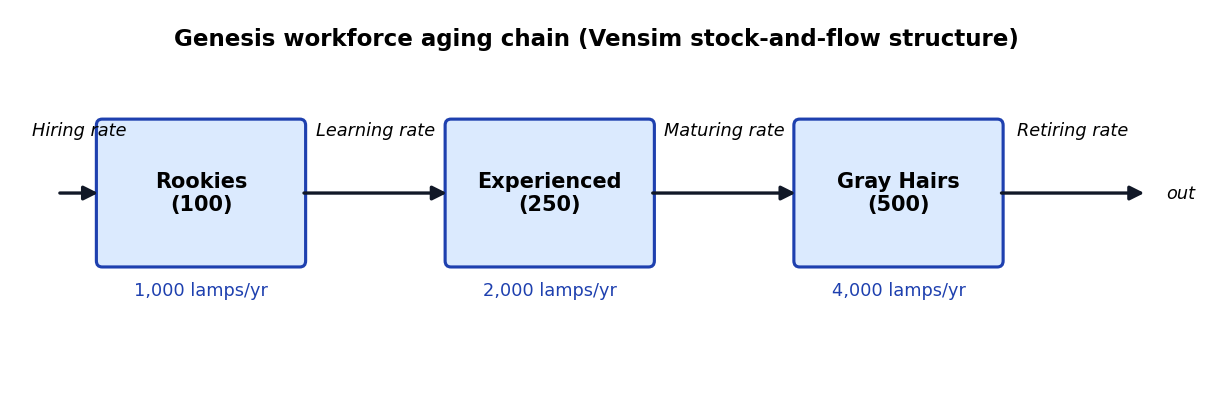
\includegraphics[width=\textwidth]{figures/fig1_schematic.png}
    \caption{Stock-and-flow structure of the Genesis workforce model. Initial
    stocks: 100 Rookies, 250 Experienced, 500 Gray Hairs (850 total).}
    \label{fig:schematic}
\end{figure}

\subsection{Equations}
With first-order (exponential) delays, the model equations are:
\begin{align*}
    \text{Rookies}(t) &= 100 + \int_0^t (\text{hiring}(s) - \text{learning}(s))\,ds \\
    \text{Experienced}(t) &= 250 + \int_0^t (\text{learning}(s) - \text{maturing}(s))\,ds \\
    \text{GrayHairs}(t) &= 500 + \int_0^t (\text{maturing}(s) - \text{retiring}(s))\,ds \\
    \text{learning} &= \text{Rookies} / T_{\text{learn}}, \quad
    \text{maturing} = \text{Experienced} / T_{\text{mat}}, \quad
    \text{retiring} = \text{GrayHairs} / T_{\text{ret}} \\
    \text{Production} &= 1000\cdot\text{Rookies} + 2000\cdot\text{Experienced}
        + 4000\cdot\text{GrayHairs} \quad \text{[lamps/year]} \\
    \text{Workforce} &= \text{Rookies} + \text{Experienced} + \text{GrayHairs}
\end{align*}
Baseline hiring is $50$/year in year~1 and $100$/year thereafter
(\texttt{50 + STEP(50,1)} in Vensim). Baseline time constants are
$T_{\text{learn}}=1$~yr, $T_{\text{mat}}=5$~yr, $T_{\text{ret}}=10$~yr.
The full Vensim equation listing is given in Appendix~A.

\subsection{Assumptions}
\begin{itemize}
    \item Transitions between tiers follow first-order delays (average times,
    not fixed pipelines).
    \item \textit{Retiring time} is the mean number of years spent as a Gray
    Hair; the retiring flow is $\text{GrayHairs}/T_{\text{ret}}$.
    \item All hires enter as Rookies; there is no attrition except retirement.
    \item Tier productivities (1,000 / 2,000 / 4,000 lamps per employee-year)
    are constant within a run; the productivity strategy of Section~6 scales
    all three by a common multiplier phased in linearly to year~10.
    \item Simulation horizon 10~years, TIME~STEP $0.0625$~yr (Euler integration).
\end{itemize}

\section{Baseline simulation}
Simulating current policy (hiring 50/year in year~1, then 100/year;
$T_{\text{learn}}=1$, $T_{\text{mat}}=5$, $T_{\text{ret}}=10$) gives, at
year~10, \textbf{1,233 employees} (100 Rookies, 457 Experienced,
676 Gray Hairs) producing \textbf{3.72~million lamps per year in total}
(Figure~\ref{fig:baseline}). Both targets are missed by a wide margin:
the workforce reaches only 73\% of its target and production only 48\% of
its target.

\begin{figure}[h]
    \centering
    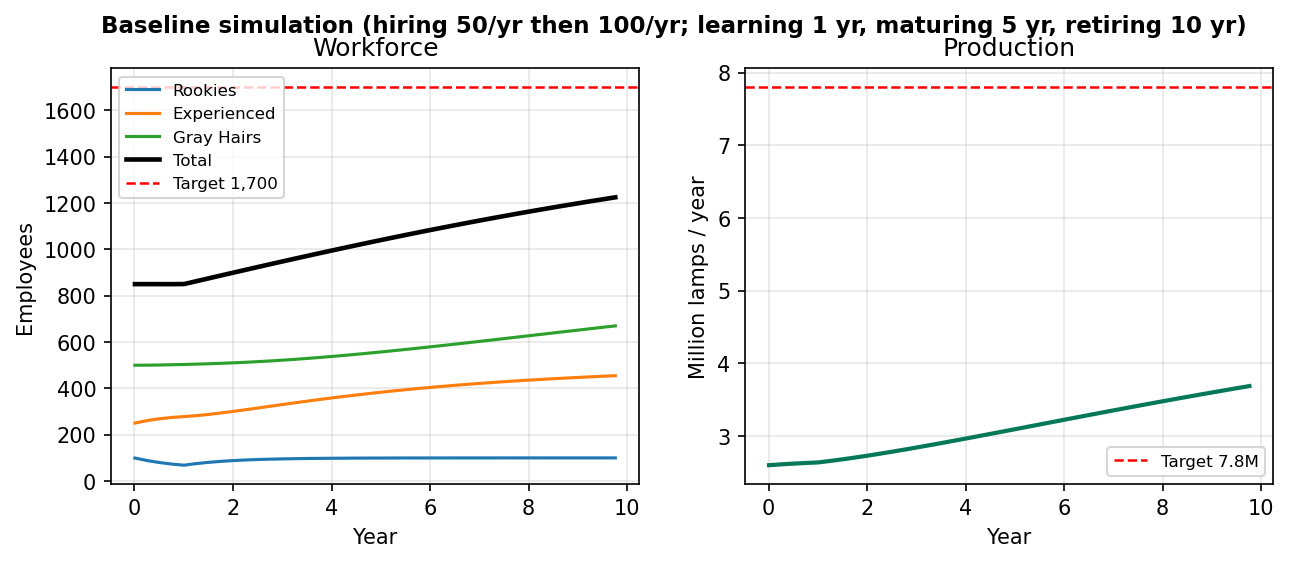
\includegraphics[width=\textwidth]{figures/fig2_baseline.png}
    \caption{Baseline trajectories. Neither the workforce target (1,700) nor
    the production target (7.8M lamps/year) is approached by year~10.}
    \label{fig:baseline}
\end{figure}

\section{Feasibility analysis}
The two targets are jointly infeasible at current productivity, independent
of any hiring policy. Producing 7.8~million lamps with 1,700 employees
requires an average output of
\begin{equation*}
    \frac{7{,}800{,}000}{1{,}700} \approx 4{,}588 \text{ lamps per employee-year},
\end{equation*}
which exceeds the 4,000 lamps per employee-year of Gray Hairs, the most
productive tier. Even if all 1,700 employees were Gray Hairs, annual output
would cap at $1{,}700 \times 4{,}000 = 6.8$~million lamps. Hence no
combination of hiring rate, learning time, maturing time, and retiring time
can meet both targets unless productivity itself rises.

\section{Experimental design}
We ran a $2^3$ factorial design on the three time constants, with levels
\begin{equation*}
    x_1 \text{ (learning): } 1\,(-),\, 2\,(+); \quad
    x_2 \text{ (maturing): } 3\,(-),\, 5\,(+); \quad
    x_3 \text{ (retiring): } 10\,(-),\, 15\,(+),
\end{equation*}
in standard order (Table~\ref{tab:design}). For each combination, the hiring
rate after year~1 was solved so that year-10 production equals exactly
7.8~million lamps at \textit{base} productivity. The production response $P$
is therefore 7.8M by construction for every row; the discriminating response
is $E$, employees at year~10.

\begin{table}[h]
    \centering
    \caption{$2^3$ design: hiring rate solved per combination to reach 7.8M
    lamps/year at base productivity. Combination~2 ($x_1=1$, $x_2=3$,
    $x_3=15$) needs the fewest employees and is the best timing combination.}
    \label{tab:design}
    \begin{tabular}{ccccccc}
        \toprule
        Combo & $x_1$ & $x_2$ & $x_3$ & Hiring/yr after yr~1 & Employees yr~10 ($E$) & Production yr~10 ($P$) \\
        \midrule
        1 & $-$ (1) & $-$ (3) & $-$ (10) & 283.2 & 2,565 & 7.8M \\
        \textbf{2} & \textbf{$-$ (1)} & \textbf{$-$ (3)} & \textbf{$+$ (15)} &
            \textbf{244.3} & \textbf{2,482} & \textbf{7.8M} \\
        3 & $-$ (1) & $+$ (5) & $-$ (10) & 293.6 & 2,784 & 7.8M \\
        4 & $-$ (1) & $+$ (5) & $+$ (15) & 258.3 & 2,687 & 7.8M \\
        5 & $+$ (2) & $-$ (3) & $-$ (10) & 303.2 & 2,810 & 7.8M \\
        6 & $+$ (2) & $-$ (3) & $+$ (15) & 264.3 & 2,701 & 7.8M \\
        7 & $+$ (2) & $+$ (5) & $-$ (10) & 315.2 & 3,030 & 7.8M \\
        8 & $+$ (2) & $+$ (5) & $+$ (15) & 279.8 & 2,912 & 7.8M \\
        \bottomrule
    \end{tabular}
\end{table}

The key finding (Figure~\ref{fig:combos}): at base productivity, reaching
7.8~million lamps requires \textbf{2,482--3,031 employees} -- overshooting
the 1,700 workforce target by 46--78\% in every combination. Faster learning
and maturing plus longer retention unambiguously help: combination~2
(1-year learning, 3-year maturing, 15-year retiring) is best on all counts,
needing the lowest hiring rate (244/year) and the fewest employees (2,482).
Hiring policy alone therefore cannot deliver both targets; productivity must
rise.

\begin{figure}[h]
    \centering
    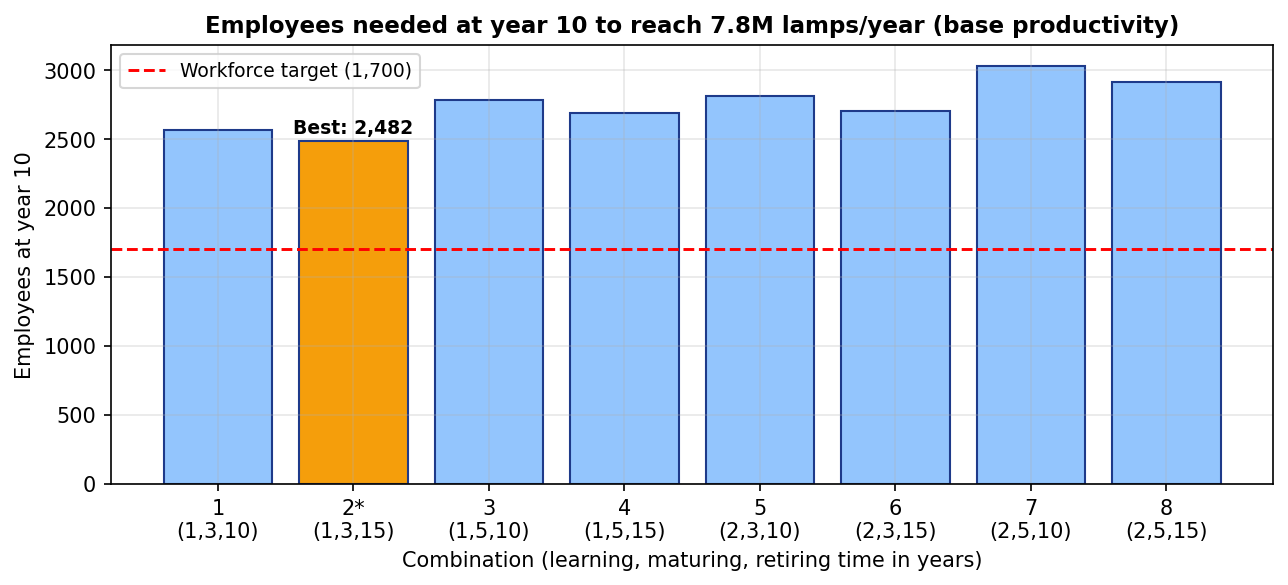
\includegraphics[width=\textwidth]{figures/fig3_combos.png}
    \caption{Employees at year~10 needed to produce 7.8M lamps/year at base
    productivity, by design combination. Every combination overshoots the
    1,700 workforce target (red dashed line); combination~2 needs the fewest.}
    \label{fig:combos}
\end{figure}

\section{Recommended strategy: pair hiring with productivity growth}
Instead of solving hiring for the production target, we now solve it for the
workforce target -- 1,700 employees at year~10 -- and compute the
productivity gain each timing combination then needs to reach 7.8~million
lamps (Table~\ref{tab:gain}).

\begin{table}[h]
    \centering
    \caption{Per-combination hiring rate for 1,700 employees at year~10, base
    production at that workforce, and required productivity gain to reach
    7.8M lamps. Combination~2 needs the smallest gain.}
    \label{tab:gain}
    \begin{tabular}{ccccc}
        \toprule
        Combo $(x_1,x_2,x_3)$ & Hiring/yr after yr~1 & Employees yr~10 &
            Base production & Required gain \\
        \midrule
        1 (1, 3, 10)  & 170.5 & 1,700 & 5.31M & +47.0\% \\
        \textbf{2 (1, 3, 15)} & \textbf{147.3} & \textbf{1,700} &
            \textbf{5.51M} & \textbf{+41.7\%} \\
        3 (1, 5, 10)  & 158.4 & 1,700 & 4.95M & +57.7\% \\
        4 (1, 5, 15)  & 139.4 & 1,700 & 5.15M & +51.3\% \\
        5 (2, 3, 10)  & 163.5 & 1,700 & 4.93M & +58.4\% \\
        6 (2, 3, 15)  & 142.9 & 1,700 & 5.15M & +51.3\% \\
        7 (2, 5, 10)  & 153.5 & 1,700 & 4.63M & +68.5\% \\
        8 (2, 5, 15)  & 136.3 & 1,700 & 4.86M & +60.6\% \\
        \bottomrule
    \end{tabular}
\end{table}

Under combination~2, hiring about \textbf{147 employees per year} (after a
first year at 50) grows the workforce to 1,700 by year~10 with base output
of 5.51~million lamps. The arithmetic linking the two targets is then direct:
\begin{equation*}
    5.51\text{M} \times 1.417 \approx 7.8\text{M},
\end{equation*}
so a \textbf{productivity gain of about 42\% by year~10} -- applied to all
tiers -- delivers both targets, and combination~2 requires the smallest such
gain of all eight tested (Figure~\ref{fig:recommended}). In practice this
gain must come from better technology, better working methods, or reduced
production cycle time.

\begin{figure}[h]
    \centering
    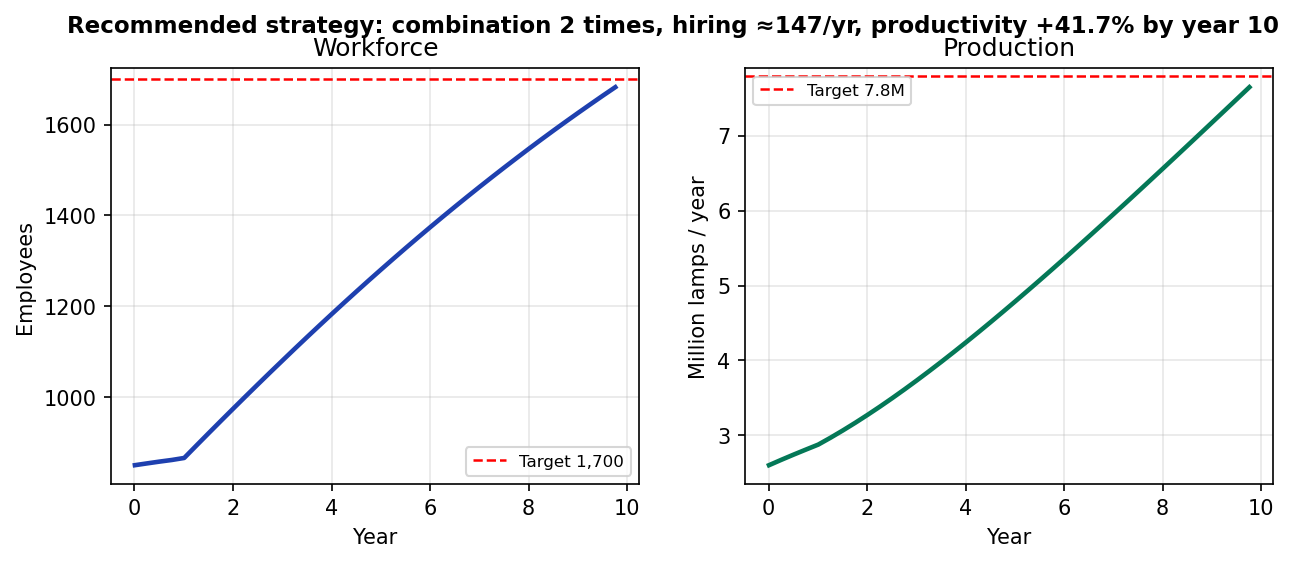
\includegraphics[width=\textwidth]{figures/fig4_recommended.png}
    \caption{Recommended strategy trajectories: combination~2 timing, hiring
    $\approx$147/year after year~1, productivity rising 41.7\% by year~10.
    Both targets are met in year~10.}
    \label{fig:recommended}
\end{figure}

\section{Model validation}
\begin{itemize}
    \item \textit{Dimensional consistency.} All stocks are in persons, flows
    in persons/year, production in lamps/year; Vensim's unit check passes.
    \item \textit{Time-step independence.} Halving TIME~STEP from 0.0625 to
    0.03125~yr changes year-10 workforce from 1,233.0 to 1,232.7 ($<$0.03\%),
    confirming the results are not a numerical artifact.
    \item \textit{Extreme conditions.} With hiring set to zero, the workforce
    decays toward zero and production follows; with productivity set to zero,
    production is zero while the workforce trajectory is unchanged. Both are
    the expected behaviors.
\end{itemize}

\section{Discussion and limitations}
The 42\% productivity gain is a \textit{requirement} derived from the model,
not a modeled mechanism: the report does not say how Genesis achieves it,
and its plausibility (new equipment, process redesign, automation) needs a
separate engineering and cost assessment, which is outside this model. Costs
of hiring, training, and retention are likewise not modeled, so the
``best'' combination is best only in workforce-efficiency terms. The
first-order delay structure is a simplification of real promotion pipelines,
and the flat hiring profile after year~1 could be refined into a phased plan.
Nevertheless, the qualitative conclusions -- the infeasibility bound, the
ranking of the timing combinations, and the necessity of productivity growth
-- are robust to these simplifications.

\section{Conclusion}
Genesis cannot reach 1,700 employees \textit{and} 7.8~million lamps per year
in ten years on hiring and workforce-aging policy alone: the production
target is provably out of reach at current productivity, and hitting it at
base productivity would require 2,482--3,031 employees. The recommended
strategy is combination~2 -- 1-year learning, 3-year maturing, 15-year
retiring -- with hiring of about 147 employees per year after the first
year and a productivity improvement of about 42\% by year~10, achieved
through technology, methods, or cycle-time reduction. This is the only tested
path that meets both ten-year targets, and it requires the smallest
productivity gain among the eight combinations examined.

\appendix
\section{Vensim equations (baseline)}
\begin{verbatim}
Rookies = INTEG(Hiring Rate - Learning Rate, 100)
Experienced = INTEG(Learning Rate - Maturing Rate, 250)
Gray Hairs = INTEG(Maturing Rate - Retiring Rate, 500)
Hiring Rate = 50 + STEP(50, 1)
Learning Rate = Rookies / Learning Time       ; Learning Time = 1
Maturing Rate = Experienced / Maturing Time   ; Maturing Time = 5
Retiring Rate = Gray Hairs / Retiring Time    ; Retiring Time = 10
Production = 1000*Rookies + 2000*Experienced + 4000*Gray Hairs
Total Employees = Rookies + Experienced + Gray Hairs
FINAL TIME = 10 ; TIME STEP = 0.0625
\end{verbatim}
\textit{Note:} the working Vensim file spells the Rookies stock and its
productivity variable ``Roockies'' and ``Productivty''; the report uses the
correct spellings throughout.

\end{document}
